\section{Diseño de Interfaz (IEEE 1016)}

El diseño de la Interfaz de Usuario (UI) y la Experiencia del Usuario (UX) constituyen un pilar crítico en este software, puesto que su propósito es educativo y debe guiar al estudiante de manera intuitiva.

\begin{figure}[ht]
\centering
\begin{tikzpicture}[
    scale=0.75, transform shape,
    node distance=1.5cm,
    screen/.style={rectangle, draw=black, thick, fill=white, minimum width=4cm, minimum height=3cm, align=center, rounded corners},
    sidebar/.style={rectangle, draw=gray, fill=gray!10, minimum width=1.2cm, minimum height=2.8cm, anchor=west},
    content/.style={rectangle, draw=blue, dashed, minimum width=2.4cm, minimum height=2.5cm, align=center, anchor=west},
    arrow/.style={->, thick, >=stealth, bend left=20}
]

% Pantalla Base
\node[screen] (app) {};
\node[sidebar] (nav) at ([xshift=0.1cm]app.west) {\rotatebox{90}{\footnotesize Menú}};
\node[content] (main) at ([xshift=1.4cm]app.west) {\footnotesize Vista \\ \footnotesize Dinámica};
\node[above=0.1cm of app] {\textbf{Estructura Base (App.jsx)}};

% Vistas
\node[screen, right=4cm of app, yshift=2cm] (view1) {Vista: \\ Título};
\node[screen, right=4cm of app, yshift=-2cm] (view2) {Vista: \\ Objetivos};
\node[screen, right=4cm of app] (view3) {...};

% Flechas de navegación
\draw[arrow] (nav.east) to node[above, sloped] {\scriptsize clic Título} (view1.west);
\draw[arrow] (nav.east) to node[below, sloped] {\scriptsize clic Objetivos} (view2.west);

\end{tikzpicture}
\caption{Diagrama de Flujo de Interfaz y Navegación Dinámica}
\label{fig:interfaz}
\end{figure}

\subsection{Principios UX/UI Aplicados}
\begin{itemize}
    \item \textbf{Carga Cognitiva Reducida:} La Figura \ref{fig:interfaz} demuestra cómo la \textit{Estructura Base} ancla un menú lateral estático, mientras que sólo la vista derecha (Vista Dinámica) cambia de contexto. Esto evita que el usuario pierda su ubicación en el sistema, ya que los módulos ("Título", "Problema") se comportan como sub-aplicaciones en una misma ventana en lugar de abrir nuevas pestañas.
    \item \textbf{Atomic CSS (Tailwind):} El diseño fue fabricado usando la filosofía de clases utilitarias de TailwindCSS. Se aplicaron colores tenues institucionales (azules y grises), tipografía sin serifas (Sans-serif) para facilitar la legibilidad prolongada, y bordes redondeados (`rounded-md`, `rounded-lg`) que comunican amabilidad en la herramienta.
    \item \textbf{Retroalimentación Constante (Feedback):} Se implementaron indicadores visuales. Al momento de generar información, el cursor del ratón cambia a \textit{not-allowed} o \textit{wait}, y los botones cambian de su tono original (Azul al 600) a un gris bloqueado (opacity-50) para impedir clics dobles accidentales.
    \item \textbf{Composición Responsiva (Mobile-First):} La estructura Base cambia su diseño usando directivas Flexbox de CSS. En una computadora de escritorio (ancho > 1024px) el menú se alinea a la izquierda (`flex-row`). Si el navegador se encoge o se accede desde un teléfono celular, el diseño colapsa hacia una columna única (`flex-col`), donde el menú se transforma en una barra de navegación en la parte superior o inferior, preservando intacta la funcionalidad táctil.
\end{itemize}

\subsection{Jerarquía de Componentes de la Interfaz (Component Tree)}

React utiliza un modelo basado en componentes donde la interfaz de usuario se construye ensamblando piezas modulares más pequeñas. El siguiente diagrama de árbol ilustra la composición arquitectónica de la vista en el navegador.

\begin{figure}[ht]
\centering
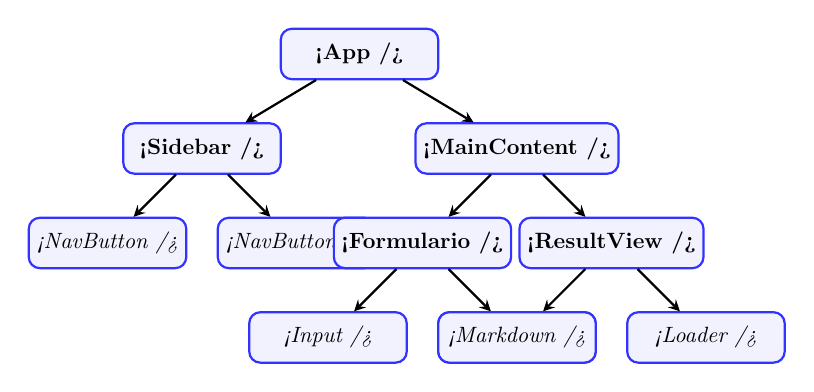
\begin{tikzpicture}[
    scale=0.8, transform shape,
    level 1/.style={sibling distance=5cm, level distance=1.5cm},
    level 2/.style={sibling distance=3cm, level distance=1.5cm},
    every node/.style={rectangle, draw=blue!80, thick, fill=blue!5, rounded corners, minimum width=2.5cm, minimum height=0.8cm, align=center},
    edge from parent/.style={draw, thick, ->, >=stealth}
]

\node (app) {\textbf{<App />}}
    child {node (sidebar) {\textbf{<Sidebar />}}
        child {node {\textit{<NavButton />}}}
        child {node {\textit{<NavButton />}}}
    }
    child {node (main) {\textbf{<MainContent />}}
        child {node (form) {\textbf{<Formulario />}}
            child {node {\textit{<Input />}}}
            child {node {\textit{<Button />}}}
        }
        child {node (result) {\textbf{<ResultView />}}
            child {node {\textit{<Markdown />}}}
            child {node {\textit{<Loader />}}}
        }
    };

\end{tikzpicture}
\caption{Árbol de Componentes de React (Jerarquía de Renderizado)}
\label{fig:jerarquia_componentes}
\end{figure}

\subsection{Explicación de la Jerarquía de Interfaz}
\begin{itemize}
    \item \textbf{Raíz (App):} El componente \texttt{<App />} es el contenedor principal (\textit{Root Node}). Su responsabilidad es manejar el Estado Global (por ejemplo, cuál pestaña está seleccionada actualmente: "Problema", "Objetivos", etc.).
    \item \textbf{Distribución de Responsabilidades:} 
    \begin{itemize}
        \item \texttt{<Sidebar />}: Componente estático o de baja volatilidad. Únicamente se encarga de renderizar la botonera de navegación. Recibe a través de \textit{Props} la función para cambiar de pestaña.
        \item \texttt{<MainContent />}: Es un componente de alta volatilidad. Dependiendo del estado global inyectado por \texttt{<App />}, decide qué formulario renderizar.
    \end{itemize}
    \item \textbf{Modularidad Atómica:} Los nodos hoja (como \texttt{<Input />}, \texttt{<Button />}, o \texttt{<Loader />}) son componentes "tontos" o presentacionales. No manejan lógica de negocio; su única misión es recibir propiedades (estilos de TailwindCSS, eventos onClick) y dibujarse en pantalla. Esta separación garantiza que el diseño de la interfaz pueda evolucionar de manera aislada sin romper la lógica de integración de la inteligencia artificial.
\end{itemize}
